\section{A 2D quasicrystal}
\subsection{Dummy}

\begin{frame}{Groundstate of the \AB\ tiling}
\(
\<{8cm}
\centering
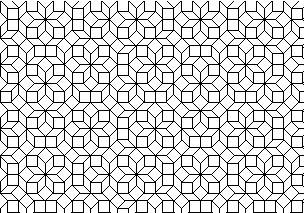
\includegraphics[width=.8\textwidth]{img/4_part3/ammann}

{\ss A patch of the \AB\ tiling}
\>
\<{7cm}
Pure hopping Hamiltonian:
\[
	\op{H} = -t\sum_{\langle m,n\rangle} \ket{m}\bra{n}
\]
Quasiperiodicity encoded in adjacency and on-site potentials
\>
\)

\textbf{Fractal} states described by \textbf{height} functions?
\[
	\psi(m) = e^{\kappa h(m)}
\]
\end{frame}

\begin{frame}{Looking for arrows}
\(
\<{7cm}
Like 1D chains, \AB\ has a substitution rule:

{\centering
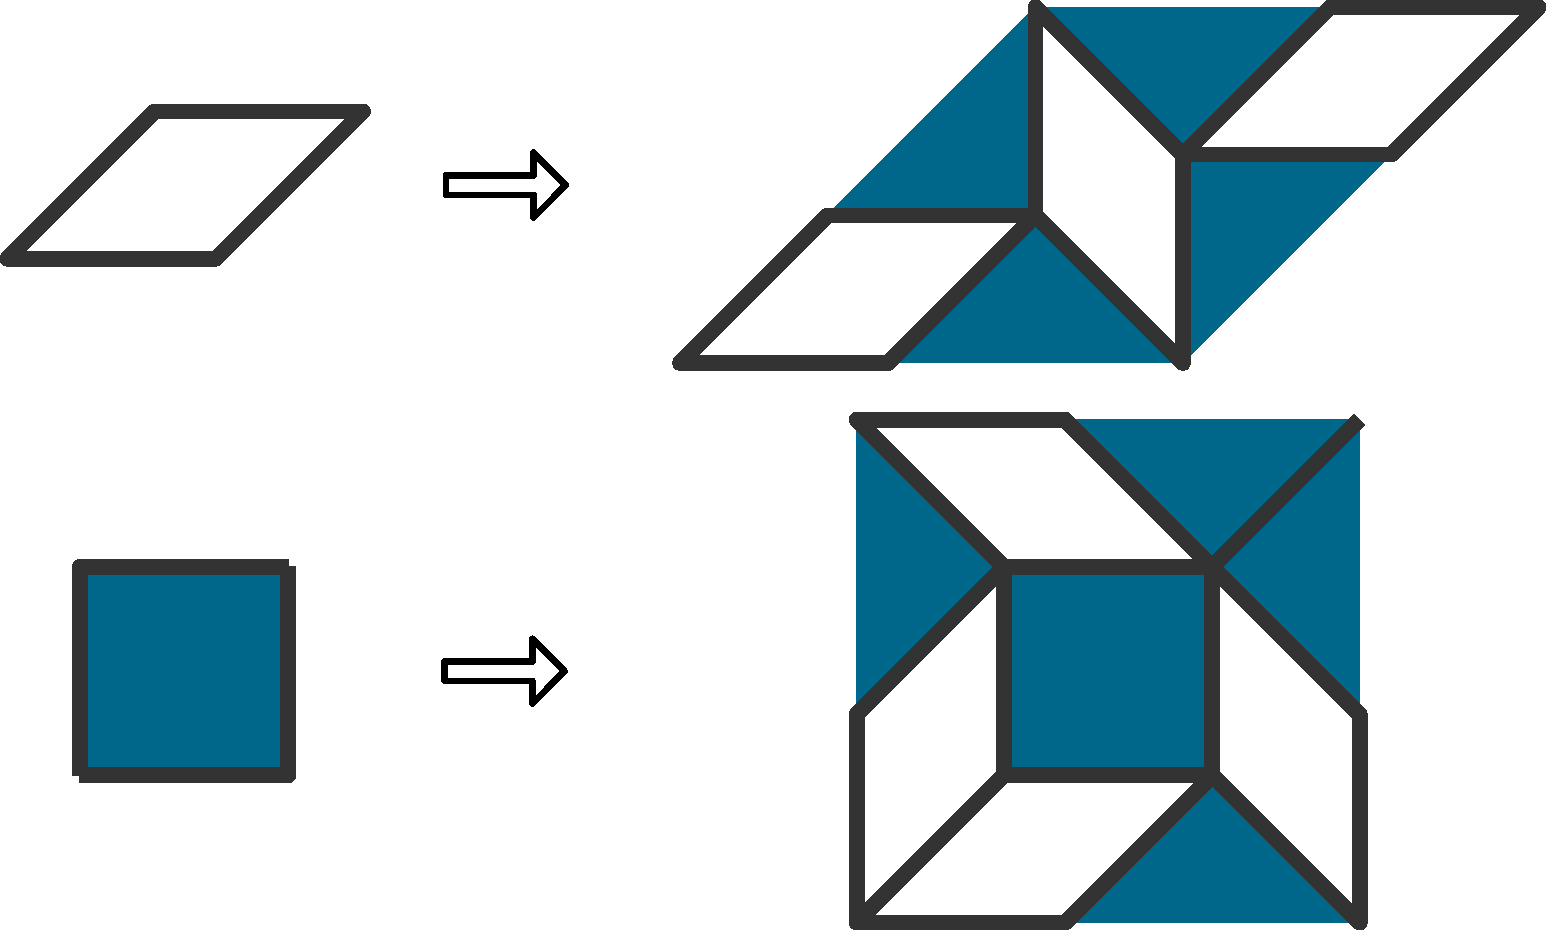
\includegraphics[width=.8\textwidth]{img/4_part3/AB_inflation}
}

$\to$ scale invariance.

Height requires a field of arrows:
\begin{itemize}
	\item invariant under substitution
	\item irrotational
\end{itemize}
\>
\<{7cm}
\AB\ $\to$ notched tiles\dots

{\centering
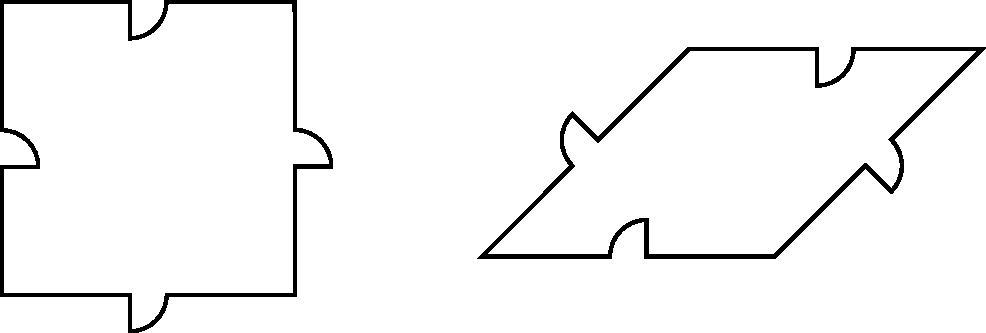
\includegraphics[width=.7\textwidth]{img/4_part3/tiles_notches}

}

\dots exactly what we need!

{\centering
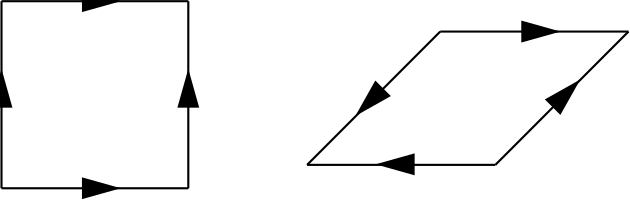
\includegraphics[width=.7\textwidth]{img/4_part3/tiles_arrows}

}

Height field:
\[
	h(m) = \sum_{0 \to m} \text{arrows}
\]
\>
\)
\end{frame}

\begin{frame}{Properties of the height field}

\(
\<{6cm}

{\centering
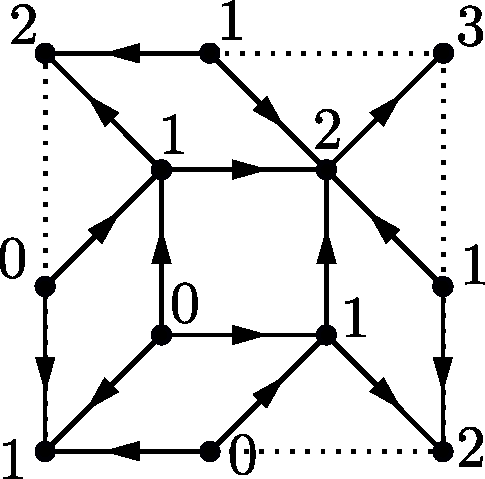
\includegraphics[width=.6\textwidth]{img/4_part3/heights_small_patch}

{\ss The height field on a small patch of the tiling.}

}

\>
\<{8cm}
{\centering
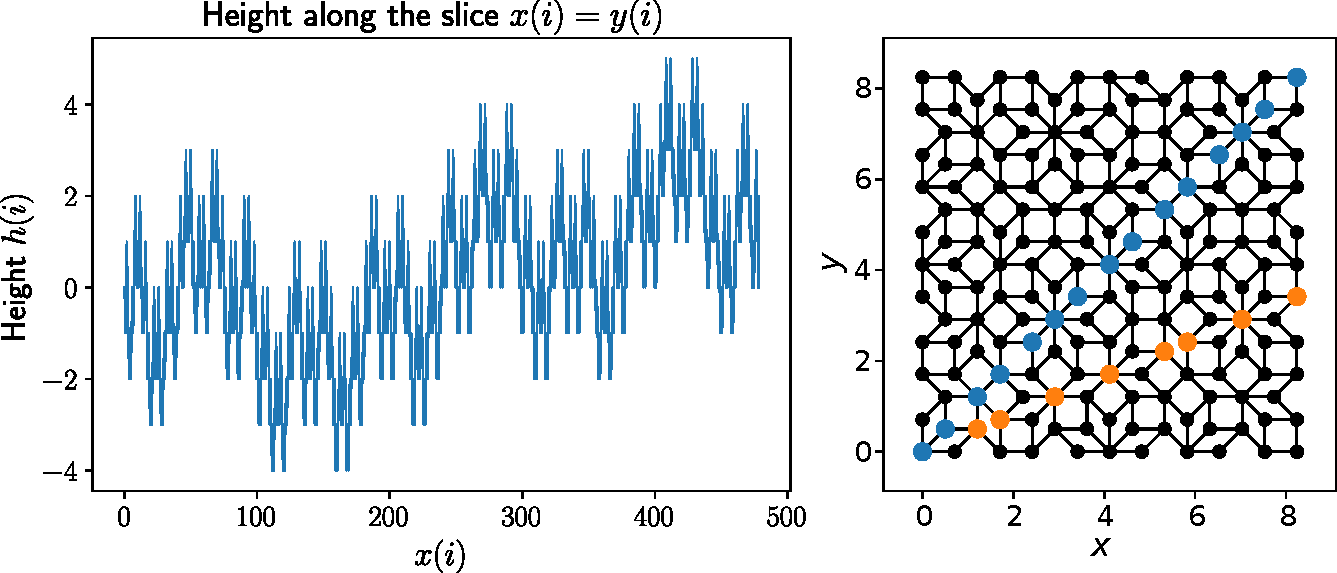
\includegraphics[width=1.\textwidth]{img/4_part3/height_combined}

{\ss Height along a line, shown in blue on the tiling.}

}

Partition function: $Z_L(\beta) \simop{L\to\infty} L^{\omega(\beta)}$

$\to$ slow growth: $h_\text{typ}(L) \simop{L\to \infty} \sqrt{\log L}$

$\to$ states $\psi(m) = e^{\kappa h(m)}$ fractal

\>
\)
\end{frame}

\begin{frame}{Groundstate}
\[
	\op{H} = -t\sum_{\langle m,n\rangle} \ket{m}\bra{n}
\]
Conjecture [Kalugin, Katz 14]:
\[
	\psi_\text{groundstate}(m) = C(m) e^{\kappa h(m)}
\]
\(
\<{7cm}
$C(m)$: \emph{local} function:

{\centering
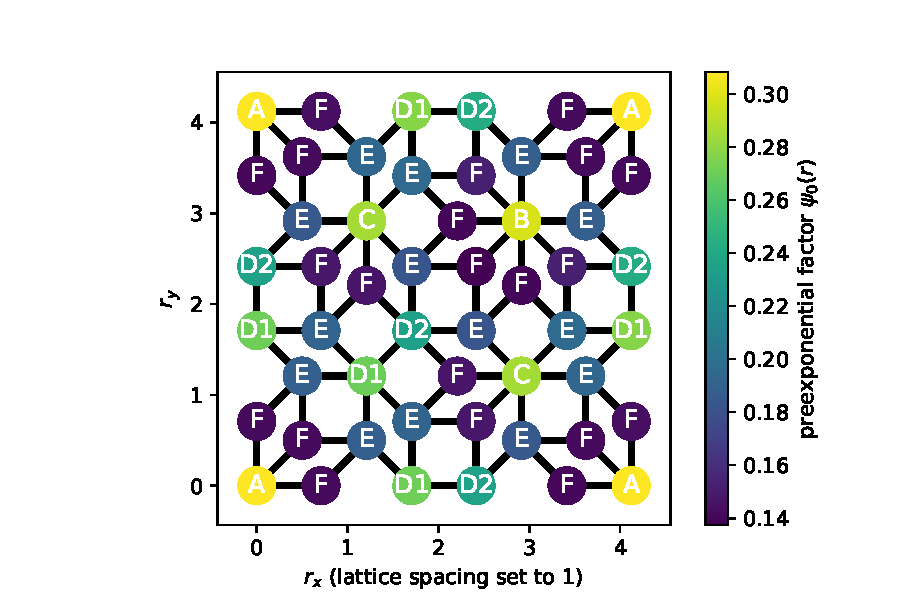
\includegraphics[width=.75\textwidth]{img/4_part3/SKK_cake_2_para}

}
\>
\<{7cm}
$e^{\kappa h(m)}$: non-local function:

{\centering
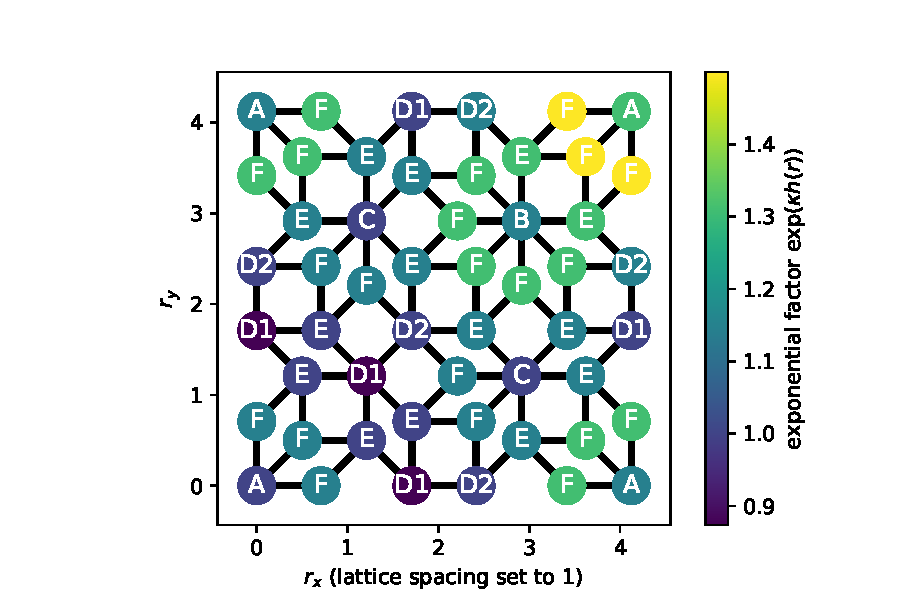
\includegraphics[width=.75\textwidth]{img/4_part3/SKK_exponential_2_para}

}

\>
\)
\end{frame}

\begin{frame}{Testing the conjecture}
Cut-and-project $\to$ physical ($E_\parallel$) and internal ($E_\perp$) space:

{\centering
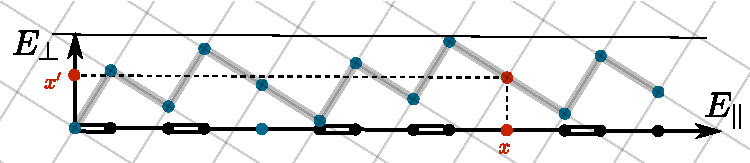
\includegraphics[width=.6\textwidth]{img/4_part3/cut_and_project_para_perp}

}
Internal space $\to$ sites classified by local environment $\to$ test the local nature of $C$:

\(
\<{7cm}
\centering
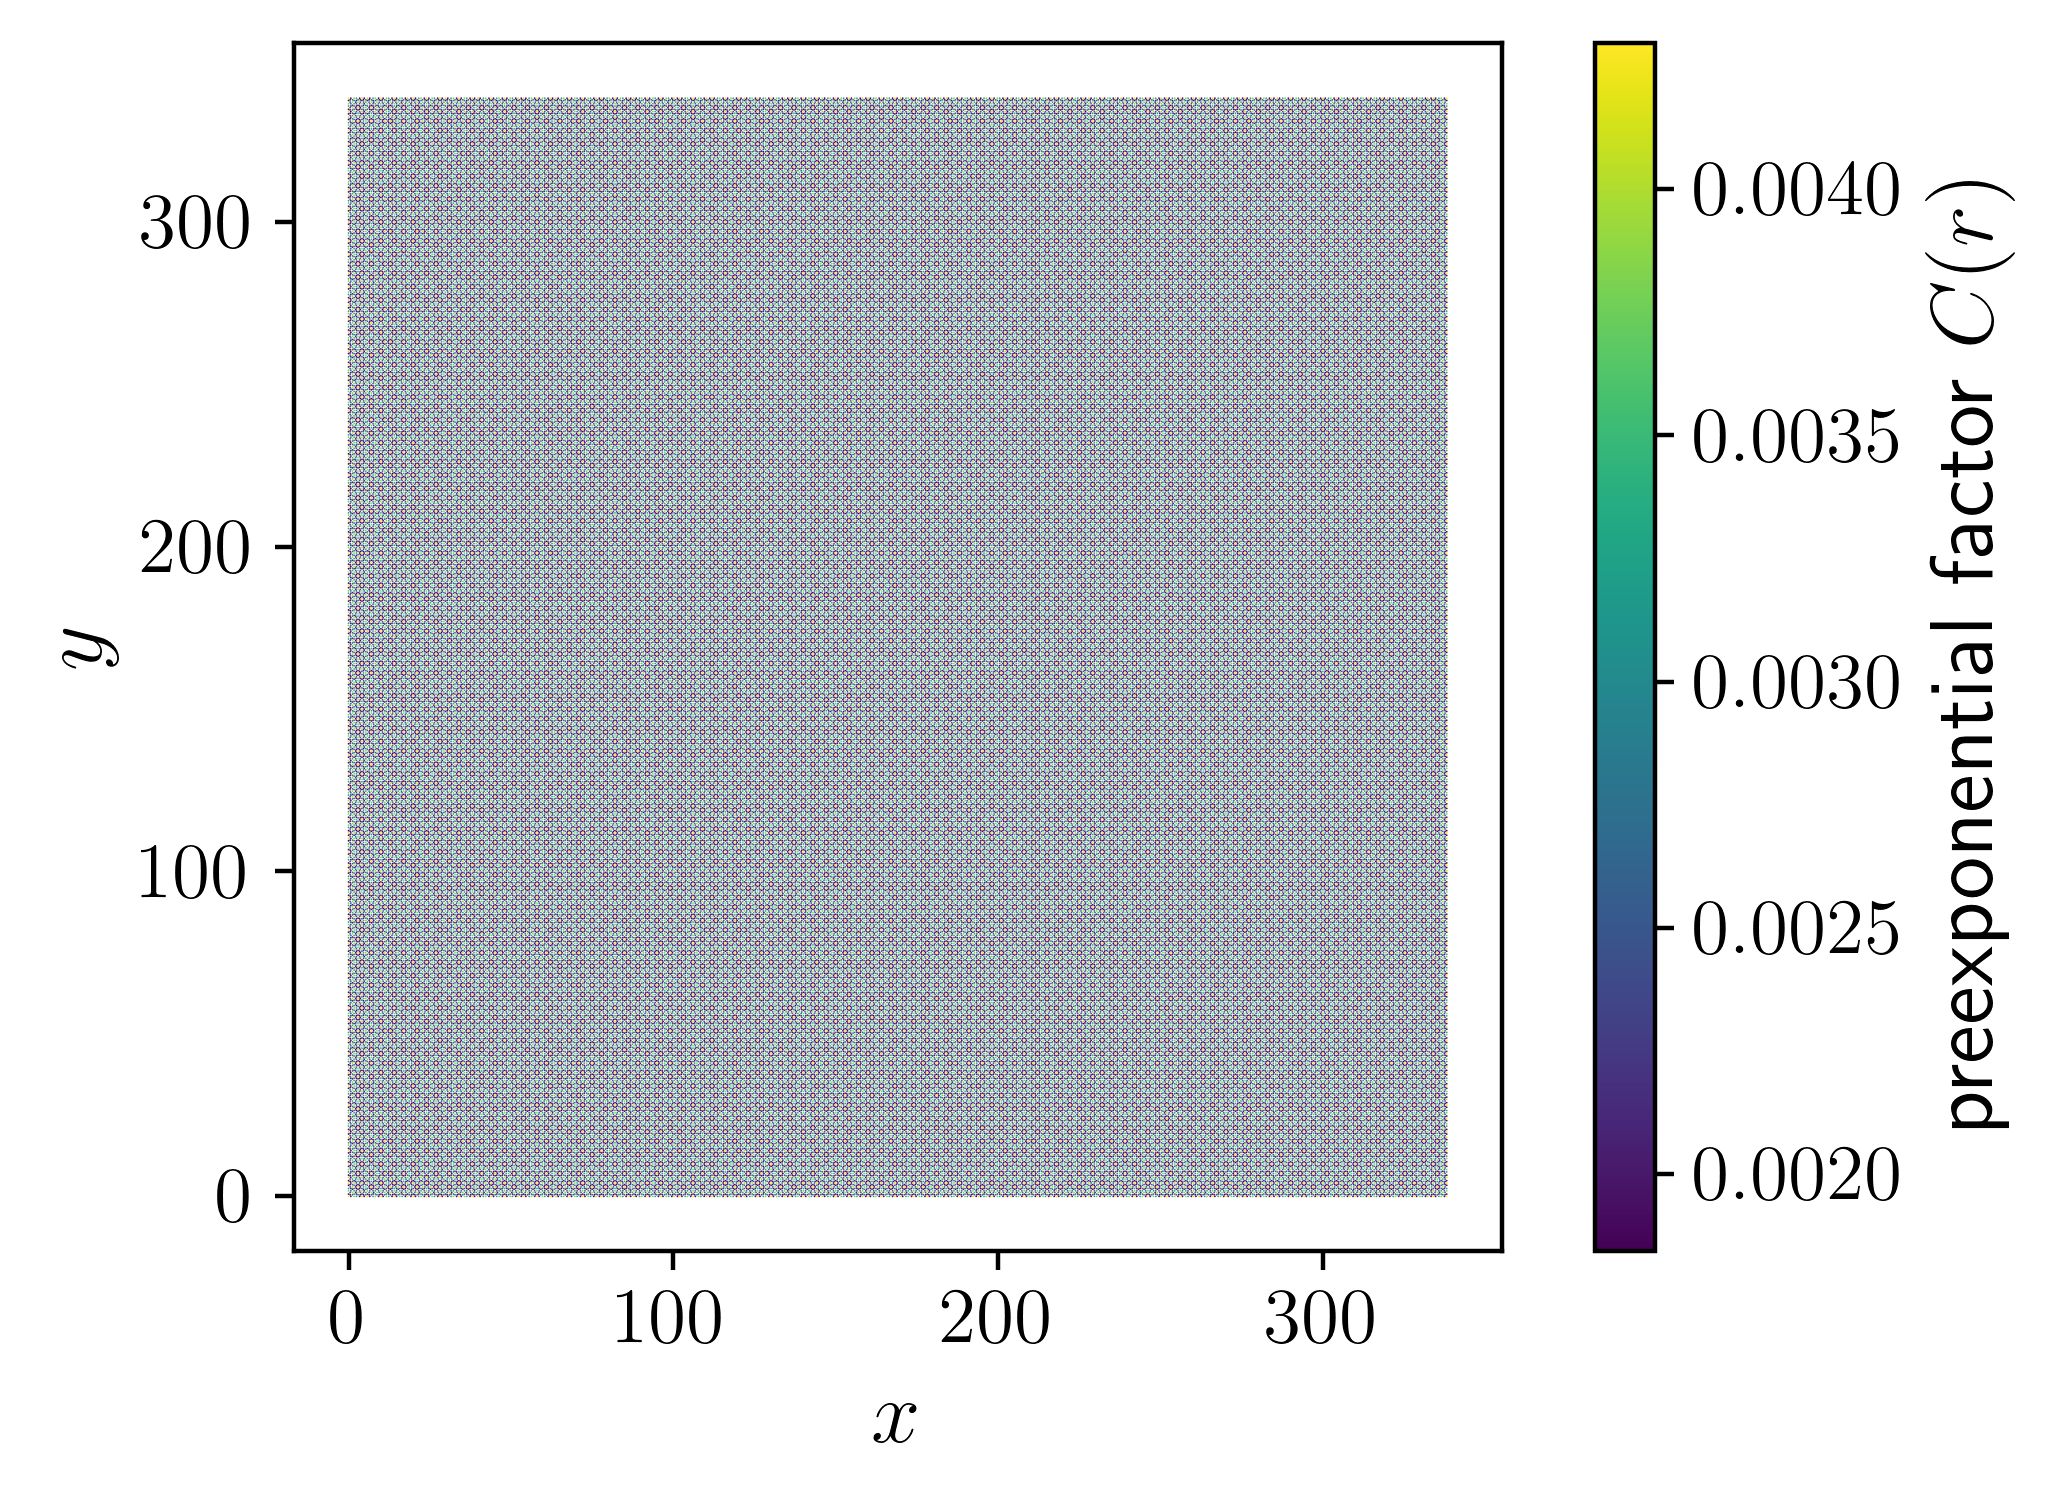
\includegraphics[width=.6\textwidth]{img/4_part3/SKK_cake_7_para}

{\ss{$C$ part in physical space (finite system of $\simeq 3 \times 10^5$ atoms)}}
\>
\<{7cm}
\centering
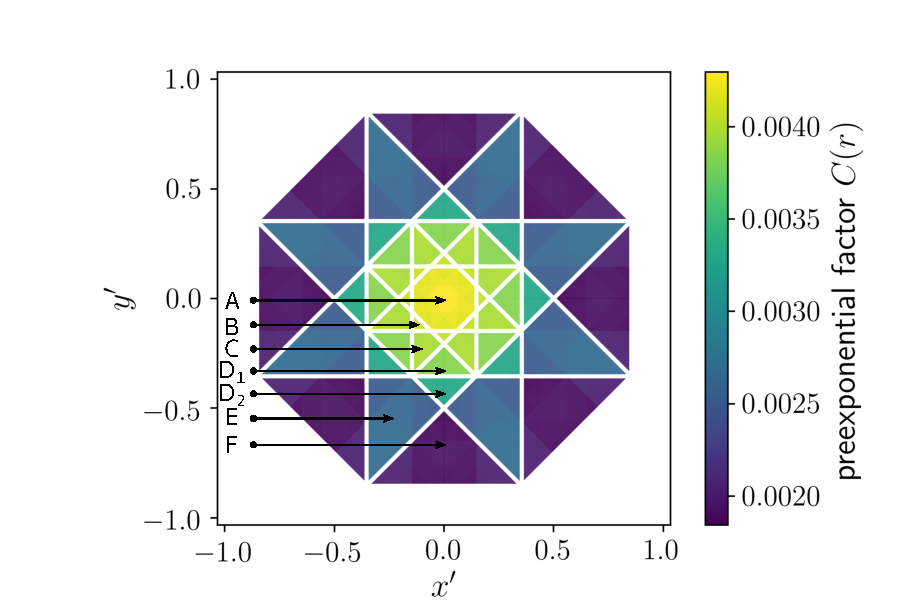
\includegraphics[width=.7\textwidth]{img/4_part3/14_SKK_cake_7_perp}

{\ss The $C$ part in internal space}
\>
\)
\end{frame}

\begin{frame}{Perturbing the Hamiltonian}
Adding an on-site potential:
\[
	\op{H} = -t\sum_{\langle m,n\rangle} \ket{m}\bra{n} + \sum_m V_m \ket{m}\bra{m}
\]
\(
\<{7cm}
Laplacian-like [Sire, Bellissard 90]:
$V_m = V z_m$

$\to$ $\psi(m) = C(m) e^{\kappa h(m)}$

{\centering
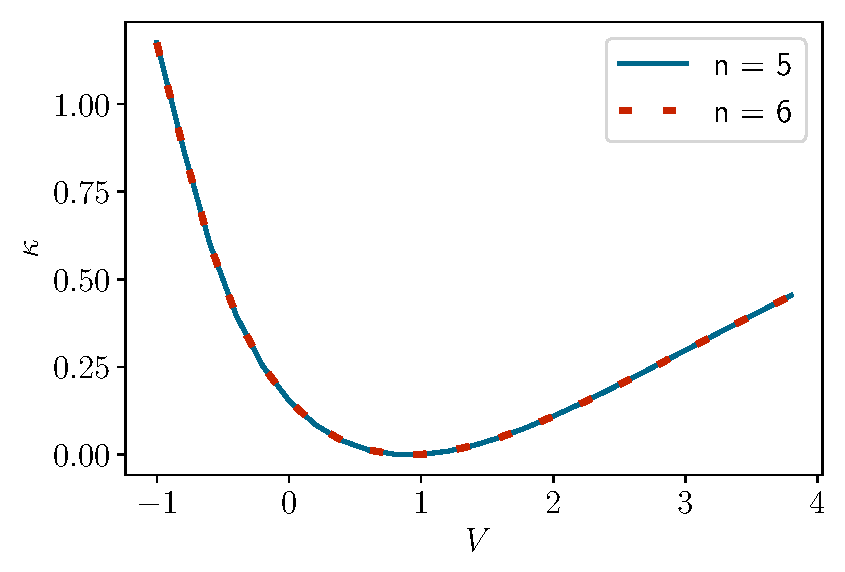
\includegraphics[width=.6\textwidth]{img/4_part3/kappa_n_5_6}

{\ss Prefactor $\kappa$ as a function of $V$.}

}

\>
\<{7cm}
An ``arbitrary'' potential:

$V_m = V$ if $m$ has 3 neighbors, else $V_m = 0$.

$\to$ $\psi(m) = C(m) e^{\kappa h(m)}$

{\centering
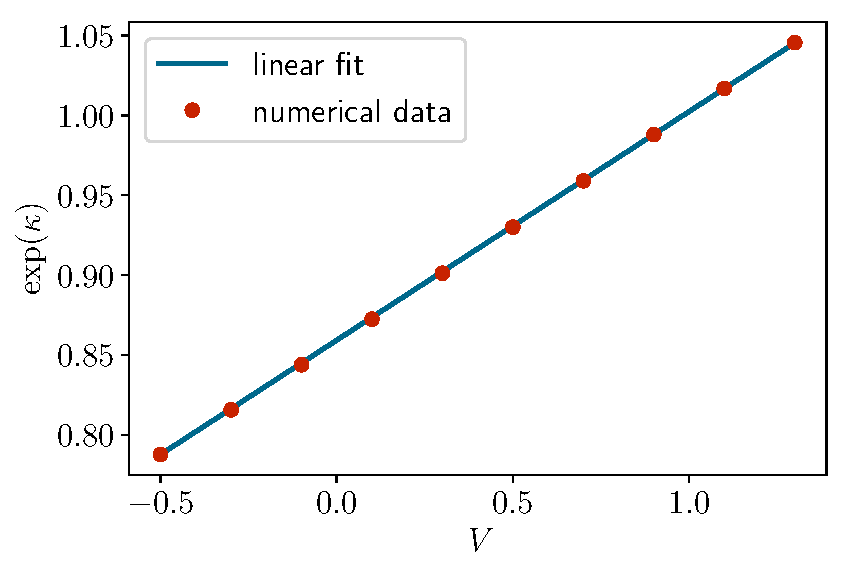
\includegraphics[width=.6\textwidth]{img/4_part3/beta_customF_ham}

{\ss{$e^{\kappa}$ as a function of $V$.}}

}

\>
\)
\end{frame}

%\begin{frame}{Fractal dimensions \& variational method}
%
%\end{frame}

\begin{frame}{Conclusions}
Tight-binding models on a 2D quasiperiodic tiling
\begin{itemize}
	\item Geometry (notches) $\to$ \textbf{height field} $h(m)$ $\to$ $\psi_\text{groundstate}(m) = C(m) e^{\kappa h(m)}$
	\item Slow height growth ($h(L) \sim \sqrt{\log L})$ $\to$ critical, \textbf{fractal} state
	\item Robust to symmetry-preserving on-site perturbations
	\item Same conclusions for the 10-fold symmetric Penrose tiling.
\end{itemize}
\end{frame}

\begin{frame}{General conclusion}
Simple tight-binding models on 1D and 2D quasiperiodic tilings
\begin{itemize}
	\item Quasiperiodic structures: in between periodic and random
	\item Critical, fractal eigenstates
	\item Consequence of quasiperiodic geometry
\end{itemize}
Perspectives
\begin{itemize}
	\item Topology: the internal space degree of freedom can be used to probe topological properties, for the Fibonacci chain [Tanese \etal{} 14]. What about 2D quasicrystals?
	\item Interactions: quasiperiodicity can be seen as a form of deterministic disorder. Although non-interacting eigenstates are not localized, many-body quasiperiodic systems seem to localize \dots how?
\end{itemize}
\end{frame}